\documentclass[a4paper]{article}
% mathematische symbolen
\usepackage{geometry}
\geometry{verbose,a4paper,tmargin=2.5cm,bmargin=2.5cm,lmargin=2.5cm,rmargin=2.5cm}
\usepackage[dutch]{babel}
\usepackage{float}
\usepackage{hyperref}
\usepackage{graphicx}
\usepackage{caption}
\usepackage{subcaption}
\usepackage{tabularx}
\usepackage{booktabs}
\usepackage{amssymb}
\usepackage{amsmath,amsthm}
\usepackage{commath}
\usepackage{latexsym}
\usepackage{amsfonts}
\usepackage{mathrsfs}
\usepackage{listings}
\renewcommand{\qedsymbol}{QED}
\theoremstyle{plain} %gebruikelijke stijl voor beweringen e.d.
\newtheorem*{vermoeden}{Vermoeden}
\newtheorem*{stelling}{Stelling}
\newtheorem*{bewering}{Bewering}
\theoremstyle{definition} %gebruikelijke stijl voor definities e.d.
\newtheorem*{definitie}{Definitie}
\newtheorem*{tegenvoorbeeld}{Tegenvoorbeeld}
\title{IN4086-14  Data Visualization: Visual Game Analytics} %vul "Herkansing" in als je een herkansing inlevert
\author{Vikko Smit\\ %nieuwe regel voor deze auteur
1293478
\and
Bastiaan Gris\`el\\
4090438
}
\begin{document}
\maketitle %produceert de daadwerkelijke titelinformatie
\section*{Introduction}
This assignment is about analyzing data from many matches for DOTA2, a MOBA-style game that went up to an impressive 8 million players worldwide last summer.\\ The game is about pushing waves of computer controlled players (NPCs) to three lanes and battle against heroes of enemy players that try to push the waves of NPCs your way.\\ Meanwhile you get a reward for killing enemy NPCs and even more for killing enemy heroes. Key aspect is this game is positioning on the playing field. You always want to stay as close as the waves of NPCs that battle each other to get gold and experience to grow in strength. However, the enemy tries to avoid you getting gold and experience so he will become more powerful. Team play is very important here, teammates can help you get rid of the enemy you play against or you can help them get an advantage in their lane. 
\section*{Problem setting}
Our focus is to make a game visualization to help people that review and comment on DOTA games to identify important moves and global activity of players. We want to achieve this by giving every player a trail of his last position and a smart detector that identifies threats in the neighborhood and notifies you where important actions are likely to be made.\\
At first, there a lot of data to be loaded and processed, this causes browsers to crash if used in one chunk. However, we don't want to limit ourselves to a small subset of the data since you might select matches that are not very interesting to see.\\
To make the data handling more robust to larger volumes we imported and indexed all locations of the players of all matches in a small mongoDB database. With this solution all data is still available and can be retrieved very fast in a web request.\\
To get a good overview you have do draw players on the map of the game. Since the dimensions of the map differs per browser / resolution setting, we chose for a solution with a grid mapped to the picture where you could enter player coordinates from the database that are instantly converted to a drawing of a dot on the respective coordinate with the respective team color.\\
This approach gives us a empty 'shell' that makes development of the visualization easier without thinking about if it would end up on the correct place.
\section*{Solution}
The data that informs us with interesting facts is divided in two parts:
\subsection*{Trail of movement}
The trail of movement is a quite simple idea: You draw a line with a fixed $\delta$t of all the positions you have been until the current time stamp. Looking at the data it is not also more clear how players move and where they are heading, but it also gives insight of the distance they run, hence distance over time is their speed. In the visualization players tend to look like snakes crawling over the battlefield.\\
It is a great tool to analyze activity of players and maybe even predict their next actions.
\subsection*{Proximity detection}
Proximity detection is a more complicated for of visualization. How to define danger and detect battles? We came up with a model that can easily be modified to fit the needs of the reviewer. To start off, we calculated the absolute distance from every player to every ally and every enemy, from now on called $d_a$ as a distance vector to all allies and $d_e$ as a distance vector to all enemies.\\
Since danger higher when you have many enemies close to you and lower when you have a lot of allies nearby, this data is normalized using $D_a = 1- \frac{d_a}{radius}$ and ofcourse the same for $d_e$.\\
These new values represent a linear relation from 0 to 1, depending if the player is at $range$ or on top of you. Distances further then $range$ are set to 0 since when players are that far away they don't count as a danger.\\
These linear values can also be transformed with for instance a square root, so the players that are very close (in range of attacking) all have a more-or-less equal danger level. To quantify "danger" you can easily take the sum of all enemies and subtract the sum of all allies, if you end up with a high value then the enemies are closer in relation to your friends and a battle of this outnumbered player might soon be happening. \\
Since you always have 1 ally close, yourself, the range of values that $D_a$ can obtain is $<1,5>$ while the range of the enemies is $<0,5>$. In total this makes the range $<-5,4>$. \\
The equilibrium in this range lies at -0.5. To get it nicely at 0 while still having a linear scale from -5 (theoretical minimum danger) to +5 (theoretical maximum danger) we apply the following formula:\\
\\
$Danger(player) = \frac{5}{4.5}(\sum{\sqrt{D_e}}-\sum{\sqrt{D_a}}+\frac{1}{2})$\\
\\
This value can be used to draw bar charts of how dangerous people are positioned at the moment in respect to the other players, but when given a arbitrarily chosen threshold this would also point out Points of Interest for the reviewer to pay some attention to. Our points of interest are players that exceed a certain threshold of positive danger. When multiple players are within the radius of the proximity detector and have a high danger value (for instance when 3 players stick together, but get attacked by 5 players of the other team) then the players are clustered to a average coordinate of the players in danger. This new virtual 'player' is then displayed as the point of interest instead of the player's individual coordinates.
\newpage
\section*{Results}
When we tested the visualization on one of the test matches (match: 569649581, time: 199, history:10 steps) we found a nice example on how these visualizations are working to their optimal. Lines give a clear indication of what just happened and what the direction and speed of the players is, while the proximity detector places circles around points that you might want to watch.
\begin{figure}[h!]
 	\centering
    	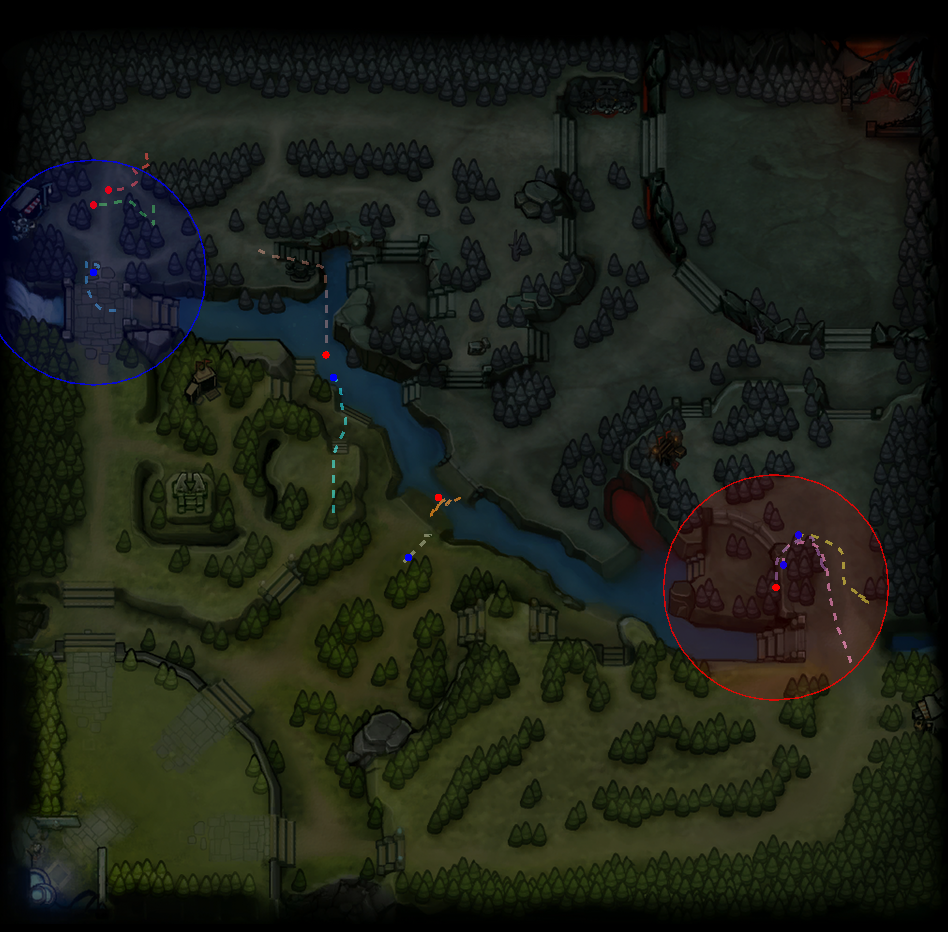
\includegraphics[width=0.5\textwidth]{proximity}
\caption*{Points of interest and trails of movement}
\end{figure}
For instance in this picture you can see the blue player in the top left being pressured in a 2vs1 standoff, while in the bottom right a red player is being chased by two opponents and is trying to get away.
Watching a few plays we haven't seen much clustering happening, but maybe if you switch to Pro games, where more teamwork is involved and people are more likely to be outnumbered in a mass vs mass battle.\\
%mongoDB database running on vikko.nl, 4GB, too big to submit, demo is running on http://datavis.vikko.nl
\end{document}





